%%%%%%%%%%%%%%%%%%%%%%%%%%%%%%%%%%%%%%%%%%%%%%%%%%%%%%%%%%%%%%%%%%%%%%
%%  Copyright by Wenliang Du.                                       %%
%%  This work is licensed under the Creative Commons                %%
%%  Attribution-NonCommercial-ShareAlike 4.0 International License. %%
%%  To view a copy of this license, visit                           %%
%%  http://creativecommons.org/licenses/by-nc-sa/4.0/.              %%
%%%%%%%%%%%%%%%%%%%%%%%%%%%%%%%%%%%%%%%%%%%%%%%%%%%%%%%%%%%%%%%%%%%%%%

\newcommand{\commonfolder}{../../common-files}
\newcommand{\webcommon}{../Web_Common}

\documentclass[11pt]{article}

\usepackage[most]{tcolorbox}
\usepackage{times}
\usepackage{epsf}
\usepackage{epsfig}
\usepackage{amsmath, alltt, amssymb, xspace}
\usepackage{wrapfig}
\usepackage{fancyhdr}
\usepackage{url}
\usepackage{verbatim}
\usepackage{fancyvrb}
\usepackage{adjustbox}
\usepackage{listings}
\usepackage{color}
\usepackage{subfigure}
\usepackage{cite}
\usepackage{sidecap}
\usepackage{pifont}
\usepackage{mdframed}
\usepackage{textcomp}
\usepackage{enumitem}
\usepackage{hyperref}


% Horizontal alignment
\topmargin      -0.50in  % distance to headers
\oddsidemargin  0.0in
\evensidemargin 0.0in
\textwidth      6.5in
\textheight     8.9in 

\newcommand{\todo}[1]{
\vspace{0.1in}
\fbox{\parbox{6in}{TODO: #1}}
\vspace{0.1in}
}


\newcommand{\unix}{{\tt Unix}\xspace}
\newcommand{\linux}{{\tt Linux}\xspace}
\newcommand{\minix}{{\tt Minix}\xspace}
\newcommand{\ubuntu}{{\tt Ubuntu}\xspace}
\newcommand{\setuid}{{\tt Set-UID}\xspace}
\newcommand{\openssl} {\texttt{openssl}}


\pagestyle{fancy}
\lhead{\bfseries SEED Labs}
\chead{}
\rhead{\small \thepage}
\lfoot{}
\cfoot{}
\rfoot{}


\definecolor{dkgreen}{rgb}{0,0.6,0}
\definecolor{gray}{rgb}{0.5,0.5,0.5}
\definecolor{mauve}{rgb}{0.58,0,0.82}
\definecolor{lightgray}{gray}{0.90}


\lstset{%
  frame=none,
  language=,
  backgroundcolor=\color{lightgray},
  aboveskip=3mm,
  belowskip=3mm,
  showstringspaces=false,
%  columns=flexible,
  basicstyle={\small\ttfamily},
  numbers=none,
  numberstyle=\tiny\color{gray},
  keywordstyle=\color{blue},
  commentstyle=\color{dkgreen},
  stringstyle=\color{mauve},
  breaklines=true,
  breakatwhitespace=true,
  tabsize=3,
  columns=fullflexible,
  keepspaces=true,
  escapeinside={(*@}{@*)}
}

\newcommand{\newnote}[1]{
\vspace{0.1in}
\noindent
\fbox{\parbox{1.0\textwidth}{\textbf{Note:} #1}}
%\vspace{0.1in}
}


%% Submission
\newcommand{\seedsubmission}{
Debe enviar un informe de laboratorio detallado, con capturas de pantalla, para describir lo que ha hecho y lo que ha observado.
También debe proporcionar una explicación a las observaciones que sean interesantes o sorprendentes.
Enumere también los fragmentos de código más importantes seguidos de una explicación. No recibirán créditos aquellos fragmentos de códigos que no sean explicados.}

%% Book
\newcommand{\seedbook}{\textit{Computer \& Internet Security: A Hands-on Approach}, 2nd
Edition, by Wenliang Du. Para más detalles \url{https://www.handsonsecurity.net}.\xspace}

%% Videos
\newcommand{\seedisvideo}{\textit{Internet Security: A Hands-on Approach},
by Wenliang Du. Para más detalles \url{https://www.handsonsecurity.net/video.html}.\xspace}

\newcommand{\seedcsvideo}{\textit{Computer Security: A Hands-on Approach},
by Wenliang Du. Para más detalles \url{https://www.handsonsecurity.net/video.html}.\xspace}

%% Lab Environment
\newcommand{\seedenvironment}{Este laboratorio ha sido testeado en nuestra imagen pre-compilada de una VM con Ubuntu 16.04, que puede ser descargada del sitio oficial de SEED.\xspace}

\newcommand{\seedenvironmentA}{Este laboratorio ha sido testeado en nuestra imagen pre-compilada de una VM con Ubuntu 16.04, que puede ser descargada del sitio oficial de SEED.\xspace}

\newcommand{\seedenvironmentB}{Este laboratorio ha sido testeado en nuestra imagen pre-compilada de una VM con Ubuntu 20.04, que puede ser descargada del sitio oficial de SEED .\xspace}

\newcommand{\seedenvironmentC}{Este laboratorio ha sido testeado en nuestra imagen pre-compilada de una VM con Ubuntu 20.04, que puede ser descargada del sitio oficial de SEED. Sin embargo, la mayoría de nuestros laboratorios pueden ser realizados en la nube para esto Ud. puede leer nuestra guía que explica como crear una VM de SEED en la nube.\xspace}

\newcommand{\seedenvironmentAB}{
Este laboratorio ha sido testeado en nuestras imagenes pre-compiladas de una VM con Ubuntu 16.04 y otra con Ubuntu 20.04, que pueden ser descargadas del sitio oficial de SEED.\xspace}

\newcommand{\nodependency}{Dado que utilizamos contenedores para configurar el entorno de laboratorio, este laboratorio no depende estrictamente de la VM de SEED. Puede hacer este laboratorio utilizando otras máquinas virtuales, máquinas físicas o máquinas virtuales en la nube.\xspace}

\newcommand{\adddns}{You do need to add the required IP address mapping to
the \texttt{/etc/hosts} file.\xspace}






\newcommand{\seedlabcopyright}[1]{
\vspace{0.1in}
\fbox{\parbox{6in}{\small Copyright \copyright\ {#1}\ \ by Wenliang Du.\\
      Este trabajo se encuentra bajo licencia Creative Commons.
       Attribution-NonCommercial-ShareAlike 4.0 International License.
       Si ud. remezcla, transforma y construye a partir de este material,
       Este aviso de derechos de autor debe dejarse intacto o reproducirse de una manera que sea razonable para el medio en el que se vuelve a publicar el trabajo.
       }}
\vspace{0.1in}
}







\lhead{\bfseries SEED Labs -- Laboratorio de Inyección SQL}

\newcommand{\sqlFigs}{./Figs}


\begin{document}


\begin{center}
{\LARGE Laboratorio de Inyección SQL }
\end{center}

\seedlabcopyright{2006 - 2020}


% *******************************************
% SECTION
% ******************************************* 
\section{Descripción General}

Una Inyección SQL es una técnica de inyección de código que explota vulnerabilidades entre la interfaz de un aplicación web y su servidor de base de datos. Esta vulnerabilidad se da cuando el input de un usuario que se envía de la aplicación web hacia el servidor back-end que conecta con la base de datos, no es validado de forma adecuada.

Muchas aplicaciones web toman el input de los usuarios para construir consultas SQL y así obtener información de la base de datos. A su vez las aplicaciones web usan consultas SQL para guardar información en la base de datos. Todas estas son prácticas comunes en el desarrollo de las aplicaciones web. Cuando una consulta SQL no es construida de manera segura, se pueden dar vulnerabilidades de Inyección SQL.
Las Inyecciones SQL son uno de los ataques más comunes en aplicaciones web.

Para este laboratorio, hemos creado una aplicación web vulnerable a un ataque de Inyección SQL. Esta aplicación incluye los errores más comunes que cometen los desarrolles web a la hora de construir aplicaciones.
El objetivo de los estudiantes es encontrar formas para explotar estas vulnerabilidades usando Inyecciones SQL, demostrar el daño que puede causar este tipo de atauqe y especializarse en las técnicas ayudan a mitigar, prevenir y evitar este tipo de ataques.
Este laboratorio cubre los siguientes tópicos:

\begin{itemize}[noitemsep]
\item Declaraciones SQL: \texttt{SELECT} y \texttt{UPDATE}
\item Inyección SQL
\item Declaraciones Preparadas (Prepared Statements)
\end{itemize}



\paragraph{Lecturas.}
Para una cobertura más detallada en Inyección SQL puede consultar:

\begin{itemize}
\item Capítulo 12 del libro de SEED, \seedbook
\end{itemize}

\paragraph{Entorno de Laboratorio.} 
\seedenvironmentB 
\nodependency


% *******************************************
% SECTION
% ******************************************* 
\section{Configuración del Entorno de Laboratorio}

Para este laboratorio hemos desarrollado una aplicación web y usaremos contenedores para configurarla. Usaremos dos contenedores, uno para la aplicación web y el otro para el servidor de base de datos para la aplicación.
La dirección IP del contenedor para la aplicación web es \texttt{10.9.0.5} y su la URL de la misma será la siguiente:

\begin{lstlisting}
http://www.seed-server.com
\end{lstlisting}

Necesitamos mapear el hostname con la dirección IP del contenedor. Por favor agregue la siguiente entrada en el archivo  \texttt{/etc/hosts}. Necesita privilegios de root para poder editar este archivo (debe usar \texttt{sudo}).
Puede ser que ya tenga agregada esta entrada de laboratorios anteriores. Si esta entrada tiene una dirección IP diferente, la entrada errónea debe de ser borrada.s

\begin{lstlisting}
10.9.0.5        www.seed-server.com
\end{lstlisting}
 

% -------------------------------------------
% SUBSECTION
% -------------------------------------------
\subsection{Setup del Contenedor y sus Comandos}

%%%%%%%%%%%%%%%%%%%%%%%%%%%%%%%%%%%%%%%%%%%%
Para empezar a preparar el contenedor, deberá descargarse el archivo \texttt{Labsetup.zip} ubicado en el laboratorio correspondiente dentro del sitio web oficial y copiarlo dentro de la Máquina Virtual prevista por SEED. Una vez descargado deberá descomprimirlo y entrar dentro del directorio \texttt{Labsetup} donde encontrará el archivo \texttt{docker-compose.yml} que servirá para setear el entorno de laboratorio. Para una información más detallada sobre el archivo \texttt{Dockerfile} y otros archivos relacionados, puede encontrarla dentro del Manual de Usuario del laboratorio en uso, en el sitio web oficial de SEED.

Si esta es su primera experiencia haciendo el setup del laboratorio usando contenedores es recomendable que lea el manual anteriormente mencionado.

A continuación, se muestran los comandos más usados en Docker y Compose.
Debido a que estos comandos serán usados con mucha frecuencia, hemos creados un conjunto de alias para los mismos, ubicados en del archivo \texttt{.bashrc} dentro de la Máquina Virtual provista por SEED (Ubuntu 20.04)

\begin{lstlisting}
$ docker-compose build  # Build the container image
$ docker-compose up     # Start the container
$ docker-compose down   # Shut down the container

// Aliases for the Compose commands above
$ dcbuild       # Alias for: docker-compose build
$ dcup          # Alias for: docker-compose up
$ dcdown        # Alias for: docker-compose down
\end{lstlisting}


Dado que todos los contenedores estarán corriendo en un segundo plano. Necesitamos correr comandos para interactuar con los mismos, una de las operaciones fundamentales es obtener una shell en el contenedor. 
Para este propósito usaremos \texttt{"docker ps"} para encontrar el ID del contenedor deseado y ingresaremos \texttt{"docker exec"} para correr una shell en ese contenedor.
Hemos creado un alias para ello dentro del archivo \texttt{.bashrc}

\begin{lstlisting}
$ dockps        // Alias for: docker ps --format "{{.ID}}  {{.Names}}" 
$ docksh <id>   // Alias for: docker exec -it <id> /bin/bash

// The following example shows how to get a shell inside hostC
$ dockps
b1004832e275  hostA-10.9.0.5
0af4ea7a3e2e  hostB-10.9.0.6
9652715c8e0a  hostC-10.9.0.7

$ docksh 96
root@9652715c8e0a:/#  

// Note: If a docker command requires a container ID, you do not need to 
//       type the entire ID string. Typing the first few characters will 
//       be sufficient, as long as they are unique among all the containers. 
\end{lstlisting}

En caso de problemas configurando el entorno, por favor consulte la sección ``Common Problems'' en el manual ofrecido por SEED. 


%%%%%%%%%%%%%%%%%%%%%%%%%%%%%%%%%%%%%%%%%%%%


% MySQL database
%%%%%%%%%%%%%%%%%%%%%%%%%%%%%%%%%%%%

\paragraph{Base de Datos MySQL.}

Los contenedores suelen ser desechables, esto quiere decir que una vez que son destruidos, toda la información dentro de ellos se pierde por completo.
Para este laboratorio queremos que nuestra información quede persistida en la base de datos MySQL, por lo tanto no perderemos nuestro trabajo al apagar nuestro contenedor. Para lograr esto, hemos montado la carpeta \texttt{mysql\_data} en nuestra Máquina Host (dentro de la carpeta \texttt{Labsetup}, esta carpeta será creada después que el contenedor de MySQL sea creado y este corriendo) ubicada en el directorio \texttt{/var/lib/mysql} dentro del contenedor MySQL, en este directorio MySQL guardará todas las bases de datos.
Inclusive si el contenedor es destruido la información de la base de datos es conservada.
Si Ud. desea resetear la base de datos puede borrar la carpeta, usando el siguiente comando;
\begin{lstlisting}
$ sudo rm -rf mysql_data
\end{lstlisting}


%%%%%%%%%%%%%%%%%%%%%%%%%%%%%%%%%%%%



% -------------------------------------------
% SUBSECTION
% -------------------------------------------
\subsection{Sobre la Aplicación Web} 

La aplicación web que hemos creado, es un simple gestor de empleados.
Los empleados pueden ver y actualizar su información personal a través de esta aplicación.
Dentro de la aplicación existen dos roles:
{\tt Administrator} que es un rol privilgiado que puede manejar la información de todos los empleados.
{\tt Employee} es un rol común y corriente que puede ver o actualizar su propia información personal. La información de los empleados se muestra en la Tabla
\ref{table:database}.

\begin{table}[htb]
\caption{Database}
\label{table:database}
\centering
\begin{adjustbox}{max width=\textwidth}
\begin{tabular}{|l|l|l|l|l|l|l|l|l|l|l|}
\hline
Name & Employee ID  & Password  &Salary  &Birthday  &SSN &Nickname &Email &Address &Phone\# \\
\hline
Admin 	& 99999       & seedadmin  &400000  &3/5   &43254314	& & & &\\
Alice 	& 10000       & seedalice  &20000   &9/20  &10211002	& & & &\\
Boby 	& 20000       & seedboby   &50000   &4/20  &10213352	& & & &\\
Ryan    & 30000       & seedryan   &90000   &4/10  &32193525	& & & &\\
Samy 	& 40000	      & seedsamy   &40000   &1/11  &32111111 	& & & &\\
Ted     & 50000	      & seedted    &110000  &11/3  &24343244	& & & &\\
\hline
\end{tabular}
\end{adjustbox}
\end{table}
 



% *******************************************
% SECTION
% ******************************************* 
\section{Tareas de Laboratorio}



% -------------------------------------------
% SUBSECTION
% ------------------------------------------- 
\subsection{Tarea 1: Conociendo las Declaraciones SQL}
\label{ssec:MySQLConsole}

El objetivo de este ataque es familiarizarse con los comandos SQL, practicando un poco con la base de datos provista. Los datos usados por nuestra aplicación web está guardada en una base de datos MYSQL que está hosteada en nuestro contenedor MySQL.
Hemos creado una base de datos llamada \texttt{sqllab\_users}, que contiene una tabla cuyo nombre es {\tt credential}. Esta tabla guarda la información personal de cada uno de los empleados (eid, password, salary, ssn,etc). En esta Tarea, la idea es que ud. practique con la base de datos y vaya familiarizándose con las consultas SQL.

Por favor obtenga una shell en el contenedor MySQL (vea el manual del contenedor para más instrucciones; este manual está en sitio oficial del laboratorio).
Use el comando \texttt{mysql} que es el cliente para conectarse a la base de datos y le servirá para interactuar con la misma desde la shell.
El usuario es {\tt root} y el password es {\tt dees}. 

	
\begin{lstlisting}
// Inside the MySQL container
# mysql -u root -pdees 
\end{lstlisting}

Después de loguearse, puede crear una base de datos nueva o cargar una ya existente. Como ya hemos creado una base de datos llamada \texttt{sqllab\_users}, solamente necesita cargarla, para hacerlo deberá de usar el comando \texttt{use}.
Para listar las tablas que componen esta base de datos puede usar el comando  \texttt{show tables} que mostrará todas las tablas que están presentes en esta base de datos.

\begin{lstlisting}
mysql> use sqllab_users;
Database changed
mysql> show tables;
+------------------------+
| Tables_in_sqllab_users |
+------------------------+
| credential             |
+------------------------+
\end{lstlisting}

Después de correr estos comandos, va a necesitar usar un comando SQL para mostrar la información personal de la empleada Alice. Por favor incluya los screenshots de sus resultados.

% -------------------------------------------
% SUBSECTION
% ------------------------------------------- 
\subsection{Tarea 2: Inyección SQL en la Declaración SELECT} 

La Inyección SQL es una técnica a través de la cual un atacante puede ejecutaruna  declaración SQL maliciosa conocida comúnmente como un payload malicioso. Por medio de este payload, los atacantes pueden robar información de la base de datos de la víctima; aún peor, pueden realizar cambios en la base de datos. Nuestra aplicación web tiene vulnerabilidades de Inyecciones SQL, que emulan los errores más comunes que comenten los desarrolladores web.

Para esta tarea, usaremos la página de login de \url{www.seed-server.com}.
La página muestra se muestra en la Figura \ref{sql:fig:login}.
Está pide al usuario ingresar su usuario y su password.
La autenticación en la aplicación esta dada por estos dos datos, solamente los empleados que tengan un usuario y password válido podrán ingresar al sistema.
Su tarea como attacante es loguearse dentro de la aplicación sin conocer las credenciales del empleado. 


\begin{figure}[htb]
\begin{center}
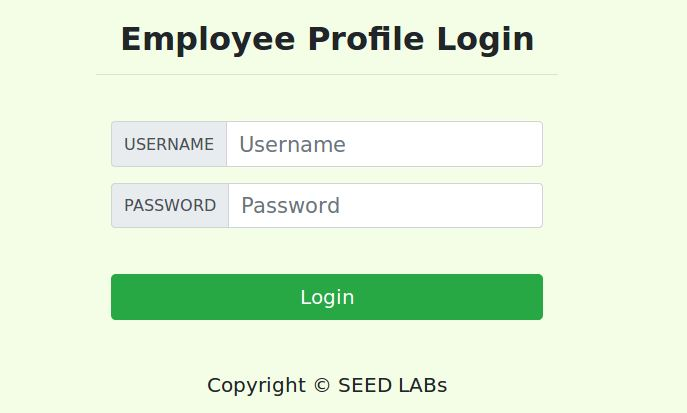
\includegraphics[width=0.7\textwidth]{\sqlFigs/login.jpg}
\end{center}
\caption{Página de Login}
\label{sql:fig:login}
\end{figure}
 
Para ayudarlo a realizar esta tarea, explicaremos como es que funciona la implementación del mecanismo de autenticación en la aplicación. El código PHP que se encarga de realizar la autenticación está en el archivo \texttt{unsafe\_home.php} dentro del directorio \path{/var/www/SQL_Injection}.
El siguiente fragmento de código muestra como los usuarios son autenticados.

\begin{lstlisting}
$input_uname = $_GET['username'];
$input_pwd = $_GET['Password'];
$hashed_pwd = sha1($input_pwd);
...
$sql = "SELECT id, name, eid, salary, birth, ssn, address, email, 
               nickname, Password
        FROM credential
        WHERE name= '$input_uname' and Password='$hashed_pwd'";
$result = $conn -> query($sql);

// The following is Pseudo Code 
if(id != NULL) {
  if(name=='admin') {
     return All employees information;
  } else if (name !=NULL){
    return employee information;
  }
} else {
  Authentication Fails;
}
\end{lstlisting}

La declaración SQL mostrada en el código, selecciona la información personal de un empleado  de la tabla {\tt credential}. Esta declaración SQL usa dos variables \texttt{input\_uname} y \texttt{hashed\_pwd}, donde \texttt{input\_uname} contiene el valor de la cadena del nombre de usuario de tipeada por el usuario en la página de login, mientras que \texttt{hashed\_pwd} contiene el hash \texttt{sha1} del password. El programa se encarga de chequear si existe algún registro que coincida con el username y password ingresado; si hay una coincidencia entonces el usuario será autenticado y se le dará su información correspondiente, de lo contrario la autenticación fallará.


\paragraph{Tarea 2.1: Ataque de Inyección SQl desde la página web.}
En esta tarea, su objetivo es loguearse en la aplicación web como administrador, de esta forma podrá ver la información de todos los empleados. Asumimos que ud. conoce el usuario del administrador el cual es {\tt admin} pero no conoce su password. Necesita decidir que ingresar como valor en los campos \texttt{Username} y \texttt{Password} para lograr un ataque exitoso.
	

\paragraph{Tarea 2.2: Ataque de Inyección SQL desde la consola.}  
En esta tarea, debe repetir lo hecho en la Tarea 2.1 pero debe hacerlo sin usar la página web. Puede usar las herramientas de la línea de comandos como puede ser \texttt{curl}, que nos sirve para enviar requests HTTP.
Cabe mencionar que si quiere incluir múltiples parametros en sus requests HTTP, necesita ponerlos en la URL dentro de un par de comillas de simples; de otra forma los caracteres especiales susados para separar los parámaetros (como \texttt{\&}) serán interpretados por la shell de una forma errónea y cambiándole el significado a lo que es la consulta dentro del aplicativo que hace los requests HTTP. El siguiente ejemplo muestra como enviar un request HTTP GET hacia nuestra aplicación web, usando dos parámetros (\texttt{username} y \texttt{Password}):

\begin{lstlisting}
$ curl 'www.seed-server.com/unsafe_home.php?username=alice&Password=11'
\end{lstlisting}

Si quiere incluir caracteres especiales en los campos de \texttt{username} o \texttt{Password}, es necesario que los codifique de forma apropiada, de lo contrario pueden cambiar el significado de su request. Si quiere incluir una comilla simple en esos campos, debería de usar \texttt{\%27}; si quiere incluir un espacio en blanco debería de usar \texttt{\%20}. En esta tarea necesita usar este tipo de codificación para enviar requests HTTP usando \texttt{curl}.


\paragraph{Tarea 2.3: Agregando una nueva declaración SQL.} 
En los ataques anteriores, solamente podemos extraer información de la base de datos; sería mucho mejor si pudieramos modificar la base de datos usando la misma vulnerabilidad en la página de login. Una idea es usar una Inyección SQL que corra dos declaraciones SQL en una sola, siendo al segunda una declaración update o delete. En SQL el punto y coma (;) es usado para separar dos declaraciones SQL. Por favor trate de correr dos declaraciones SQL usando la página de login.

Existe una contramedida para prevenir que se puedan correr dos declaraciones SQL en este ataque. Por favor use el libro de SEED o algún recurso de Internet para descubrir cual es esta contramedida y agregue su descubrimiento en el informe del laboratorio.


% -------------------------------------------
% SUBSECTION
% ------------------------------------------- 
\subsection{Tarea 3: Inyección SQL en la Declaración UPDATE} 

Si la Inyección SQL incluye una declaración UPDATE, el daño que puede ocasionar podría ser severo, los atacantes pueden usar esto para modificar la base de datos.
En nuestra aplicación, existe una página de edición de perfil (Figura    \ref{sql:fig:edit}) esto le permite a los empleados actualizar su información de perfil, incluyendo su nickname, email, address, phone, number and password. Para visitar esta página los empleados primero necesitan estar logueados.

Cuando los empleados actualizan su información a través de esta página de edición de perfil, la siguiente consulta SQL UPDATE será ejecutada. El código PHP que implementa esta actualización del perfil del empleado está en el archivo {\tt unsafe\_edit\_backend.php} dentro del directorio {\tt /var/www/SQLInjection}.


\begin{lstlisting}
$hashed_pwd = sha1($input_pwd);
$sql = "UPDATE credential SET
	nickname='$input_nickname',
	email='$input_email',
	address='$input_address',
	Password='$hashed_pwd',
	PhoneNumber='$input_phonenumber'
	WHERE ID=$id;";
$conn->query($sql);
\end{lstlisting}
 

\begin{figure}[htb]
\begin{center}
  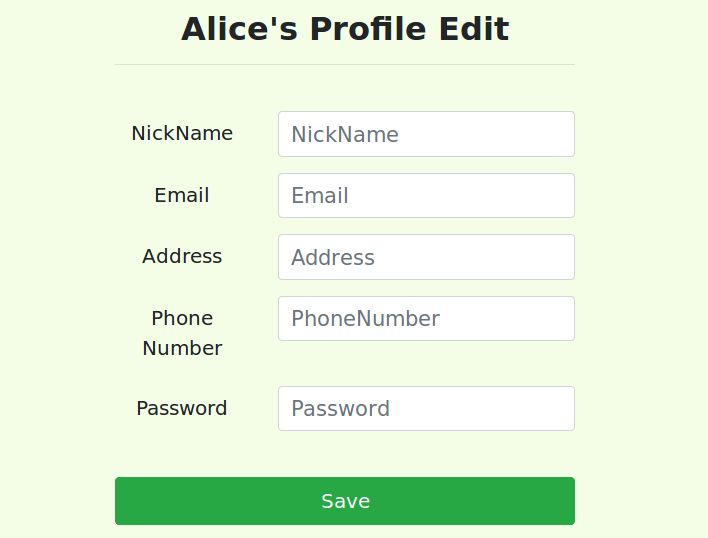
\includegraphics[width=0.6\textwidth]{\sqlFigs/editprofile.jpg}
\end{center}
\caption{Página de Edición del Perfil}
\label{sql:fig:edit}
\end{figure}
 


\paragraph{Tarea 3.1: Modificar su propio salario.}  
Como se mostró en la página de edición del perfil, los empleados sólo pueden actualizar su nickname, emails, addresses, phone numbers y passwords; no están autorizados para cambiar sus salarios.
Asuma que ud. (Alice) es una empleada descontenta y su jefe Boby no le ha dado un aumento en lo que va del año. Ud. quiere incrementar su salario y lo hará explotando una vulnerabilidad a través de una Inyección SQL en la página de edición de su perfil. Por favor demuestre como puede lograr esto.
Asumimos que ud. no sabe que los salarios son guardados en una columna llamada \texttt{salary} dentro de la base de datos.


\paragraph{Tarea 3.2: Modificar el salario de otras personas.}
Después de incrementar su propio salario. ud. decide castigar a su jefe Boby, reduciendo su salario en 1 dolar. Por favor demuestre como puede lograr esto.

\paragraph{Tarea 3.3: Modificar el password de otras personas.}
Después de cambiar el salario de Boby, ud. sigue descontenta, y quiere cambiar el password de Boby a un password que ud. conoce, para así podeer acceder a la cuenta de Boby en el sistema y hacer mucho más daño. Por favoor demuestre como puede lograr esto.
Necesita mostrar que puede loguearse de forma exitosa en la cuenta de Boby usando el nuevo password. 
Una cosa que cabe mencionar es que la base de datos almacena el hash del password y no su valor en texto plano. Puede hechar un vistazo nuevamente al código que se encarga de realizar este cambio {\tt unsafe\_edit\_backend.php} y validar como se está guardando el password. Se usa la función de hashing SHA1 para generar el valor del passsword.




\subsection{Tarea 4: Contramedida --- Declaraciones Preparadas} 

El problema fundamental de las vulnerabilidades de Inyección SQL es que se falla en separar los datos del código. Cuando se construye una declaración SQL, el programa (en este caso nuestro programa PHP) sabe cuales son los datos y cual es el código. 
Desafortunadamente, cuando la declaración SQL es enviada a la base de datos, esta diferenciación desaparece; los límites que el interprete de SQL entiende difieren de los interpretados originalmente por el desarrollador en el código de la aplicación.
Para resolver este problema, es importante asegurarse que tanto el código del servidor que representa nuestra aplicación y la base de datos interpreten lo mismo. La forma más segura de asegurarse de esto es a través de las \textit{declaraciones preparadas o prepared statements}. 

\begin{figure}
\centering

\includegraphics[width=0.8\textwidth]{\sqlFigs/PreparedStatement.pdf}
\caption{Workflow de las Declaraciones Preparadas o Prepared Statements}
\label{sql:fig:preparedstatement}
\end{figure}

Para entender como las declaraciones preparadas nos ayudan a prevenir Inyecciones SQL, necesitamos entender que ocurre cuando un servidor SQL recibe una consulta.
En la Figura \ref{sql:fig:preparedstatement} se muestra un diagrama de alto nivel que explica como son ejecutadas las consultas.
En la fase de compilación, las consultas pasan por un proceso de parseo y normalización, donde se chequea su semántica y sintáctica
La siguiente fase es la compilación donde palabras como (SELECT, FROM, UPDATE, etc) son convertidas en un formato entendible para las máquinas. Básicamente en esta etapa la consulta es interpretada.
En la fase de la optimización de la consulta, son consideradas diversas estrategias o planes para ejecutar la consulta de la forma más óptima posible. Estos planes son guardados en una cache en el motor de base de datos, por lo que sí llega la misma consulta esta será buscada dentro de esa cache y si es encontrada se evitarán las fases de parseo, compilación y optimización. Finalmente la consulta compilada pasa por la fase de ejecución donde se termina de ejecutar por completo.

Las declaraciones preparadas entran en juego después de la compilación pero antes de la ejecución.
Una declaración preparada pasará por la fase de compilación y será convertida en una consulta pre-compilada con una serie de marcadores que estarán vacíos para los datos. Para correr la consulta pre-compilada los datos deben de ser provistos pero estos datos no pasarán por la fase de compilación; en su lugar irán conectados directamente en la consulta pre-compilada y serán enviados al motor de ejecución.
Es más, si hay código SQL dentro de los datos, este código será evaluado como si fuese un dato más, sin ningún tipo de significado especial.
Así es como las declaraciones preparadas nos previenen de posibles ataques de Inyección SQL.

A continuación mostraremos un ejemplo de como escribir una declaración preparada en PHP. Usamos una declaración SELECT en el código y mostramos como usar una declaración preparada en un código vulnerable a una Inyección SQL.


\begin{lstlisting}
$sql = "SELECT name, local, gender  
        FROM USER_TABLE 
        WHERE id = $id AND password ='$pwd' ";
$result = $conn->query($sql)
\end{lstlisting}

El código mostrado anteriormente es vulnerable a un ataque de Inyección SQL.
Puede ser reescrito de la siguiente forma


\begin{lstlisting}
$stmt = $conn->prepare("SELECT name, local, gender
                        FROM USER_TABLE 
                        WHERE id = ? and password = ? ");
// Bind parameters to the query
$stmt->bind_param("is", $id, $pwd);
$stmt->execute();
$stmt->bind_result($bind_name, $bind_local, $bind_gender);
$stmt->fetch();
\end{lstlisting}

Usando el mecanismo de la declaración preparada, dividimos el proceso de enviar declaraciones SQL a la base de datos en dos pasos.
El primer paso es enviar la parte del código (es decir la declaración SQL sin los datos), esto se hace por medio del prepare y se puede observar en el fragmento del código anterior, los datos de la consulta son reemplazados por un signo de pregunta (?). Después de este paso, enviamos los datos a la base de datos usando {\tt bind\_param()} que se encarga de enlazarlos por medio de los signos de pregunta a sus valores equivalentes de la declaración preparada.
La base de datos interpretará y tratará todo lo que se envie de esta forma como datos y no como código. 
En el método {\tt bind\_param()}, el primer argumento {\tt "is"} indica los tipos de los parámetros: \texttt{"i"} es para un tipo de dato entero en este caso {\tt \$id} y \texttt{"s"} es para un tipo de dato de cadena en este caso {\tt \$pwd}.

\paragraph{Tarea.} En esta tarea, usaremos el mecanismo de declaración preparada para arreglar las vulnerabilidades de Inyeccion SQL. Para hacerlo más sencillo, hemos simplificado el programa dentro del directorio \texttt{defense}. Haremos los cambios sobre los archivos dentro de este directorio.
Si ud. apunta su navegador hacia esta URL, verá una página similar a la de login de la aplicación web. Esta página le permite consultar la información de un empleado pero debe de ingresar el username y el password correcto.


\begin{lstlisting}
URL: http://www.seed-server.com/defense/
\end{lstlisting}

Los datos ingresados en esta página serán enviados al programa servidor \texttt{getinfo.php} que invocará un programa llamado \texttt{unsafe.php}.
La consulta SQL dentro de este programa PHP es vulnerable a un ataque de Inyección SQL. Su tarea es modificar la consulta SQL usando una declaración preparada dentro de \texttt{unsafe.php} y proteger al programa contra este tipo de ataque.
Dentro del directorio del setup del laboratorio, el archivo \texttt{unsafe.php} está ubicado en el directorio \path{image_www/Code/defense}. Puede modificar el archivo directamente desde ahí y una vez terminado, necesita reconstruir y reiniciar el contenedor o los cambios no tendrán efecto.

También puede modificar el archivo mientras el contenedor está corriendo.
En el contenedor corriendo el archivo \texttt{unsafe.php} se encuentra dentro de \path{/var/www/SQL_Injection/defense}.
La desventaja de esto es que para mantener el tamaño de la imagen del docker pequeña hemos instalado dentro del contenedor, un editor de texto bastante simple llamado \texttt{nano}, si bien este editor debería de ser suficiente para realizar esta tarea, si ud. prefiere instalar otro editor con el que se sienta más a gusto debe usar \texttt{"apt install"} desde la consola para instalarlo. Por ejemplo para instalar \texttt{vim} podemos hacer lo siguiente:

\begin{lstlisting}
# apt install -y vim 
\end{lstlisting}

Esta instalación será descartada una vez que el contenedor es apagado y destruido.
Si quiere hacer esta instalación permanente debería de agregar el comando de instalación en el archivo \texttt{Dockerfile} ubicado en el directorio  \path{image_www}. 


\section{Guías}
\label{sec:guidelines}

\paragraph{Probando Cadena de Inyección SQL.}
En aplicaciones del mundo real, puede ser difícil chequear cuando un ataque de Inyección SQL contiene un error de sintáxis, generalmente los servidores no devuelven este tipo mensajes de error.
Para llevar a cabo esta investigación, puede copiar la declaración SQL del código PHP en la consola MySQL. Asuma que tiene la siguiente declaración SQL y la cadena para hacer la inyección es {\tt ' or 1=1;\#}. 

\begin{lstlisting}
SELECT * from credential 
WHERE name='$name' and password='$pwd';
\end{lstlisting}

Puede reemplazar el valor de {\tt \$name} con la cadena de inyección provista anteriormente y probarla en la consola MySQL.
Esto le ayudará a crear cadenas de Inyección SQL sin errores de sintaxis antes de llevar a cabo ataques en un escenario real.



% *******************************************
% SECTION
% ******************************************* 
\section{Informe del Laboratorio}


%%%%%%%%%%%%%%%%%%%%%%%%%%%%%%%%%%%%%%%%

Debe enviar un informe de laboratorio detallado, con capturas de pantalla, para describir lo que ha hecho y lo que ha observado.
También debe proporcionar una explicación a las observaciones que sean interesantes o sorprendentes.
Enumere también los fragmentos de código más importantes seguidos de una explicación. No recibirán créditos aquellos fragmentos de códigos que no sean explicados.
%%%%%%%%%%%%%%%%%%%%%%%%%%%%%%%%%%%%%%%%


% *******************************************
% SECTION
% *******************************************
\section*{Agradecimientos}

Este documento ha sido traducido al Español por Facundo Fontana


\end{document}


%%%%%%%%%%%%%%%%%%%%%%%%%%%%%%%%%%%%%%%%%%%%%
%%%%%%%%%%%%%%%%%%%%%%%%%%%%%%%%%%%%%%%%%%%%%
%%%%%%%%%%%%%%%%%%%%%%%%%%%%%%%%%%%%%%%%%%%%%
%%%%%%%%%%%%%%%%%%%%%%%%%%%%%%%%%%%%%%%%%%%%%
%%%%%%%%%%%%%%%%%%%%%%%%%%%%%%%%%%%%%%%%%%%%%





% This part is removed 
\begin{comment}
\paragraph{Escaping Special Characters using magic\_quotes\_gpc}

You will get to know that SQL Injection attack is possible because of attacker can use some
special character to alter the existing SQL queries.  In the PHP code, if a data variable is a
string type, it needs to be enclosed within a pair of single quote (').  For example, in the
SQL query listed above, we have used {\tt name = `\$user'}.  The single quote symbol
surrounding {\tt \$user} basically “tries” to separate the data in the {\tt \$user} variable
from the code.  Unfortunately, this separation will fail if the content of {\tt \$user}
variable include any single quote.  Therefore, we need a mechanism to tell the database that
the single quote in {\tt \$user} should be treated as a part of the data, not like the special
character in SQL.  All we need to do is to add a backslash (\textbackslash) before the single
quote, which will prevent us to alter any existing SQL query.  PHP provides a mechanism to
automatically add a backslash before single-quote ('), double quote ("), backslash
(\textbackslash), and NULL characters.  If this mechanism is turned on, all of these characters
in the user inputs will be automatically escaped.  This mechanism is known as magical quotes
and generally refer by the value of {\tt magic\_quotes\_gpc}.

 
Please note that, magic\_quotes\_gpc feature has been DEPRECATE as of 5.3.0 and REMOVED as of
PHP 5.4.0.  The PHP version installed in SEEDUbuntu VM is 5.3.5, so you can still play with
this. The reasons why it is removed is described below:

\begin{itemize}
\item Portability: Assuming it to be on, or off, affects portability.
Most code has to use a function called {\tt get\_magic\_quotes\_gpc()} to check for this,
and code accordingly.

\item Performance and Inconvenience: Not all user inputs are used
for SQL queries, so mandatory escaping all data not only affects
performance, but also become annoying when some data are not
supposed to be escaped.
\end{itemize}

\end{comment}
